\chapter{CE Declarations}
\label{annexdeclarations}
 
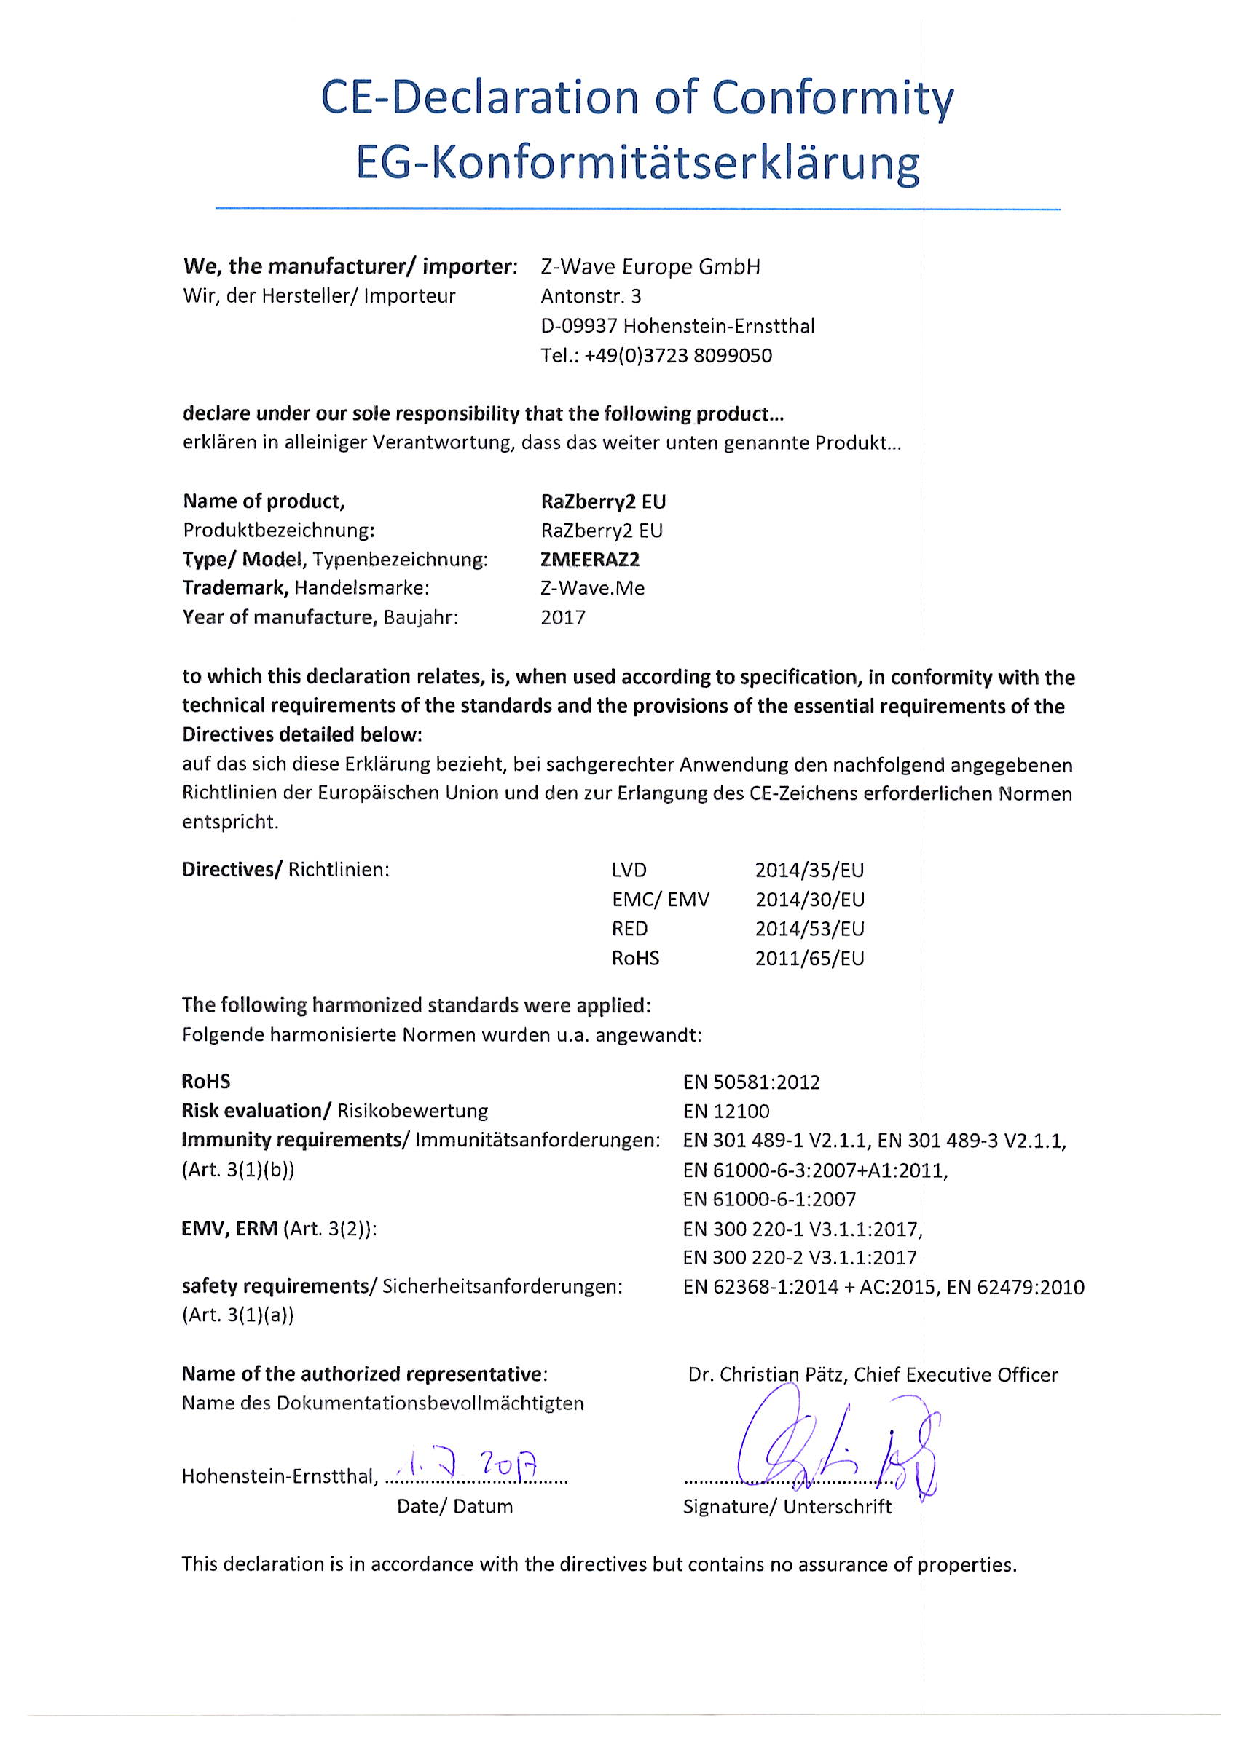
\includegraphics[width=0.9\textwidth]{pdfs/CE_RAZ2.pdf}

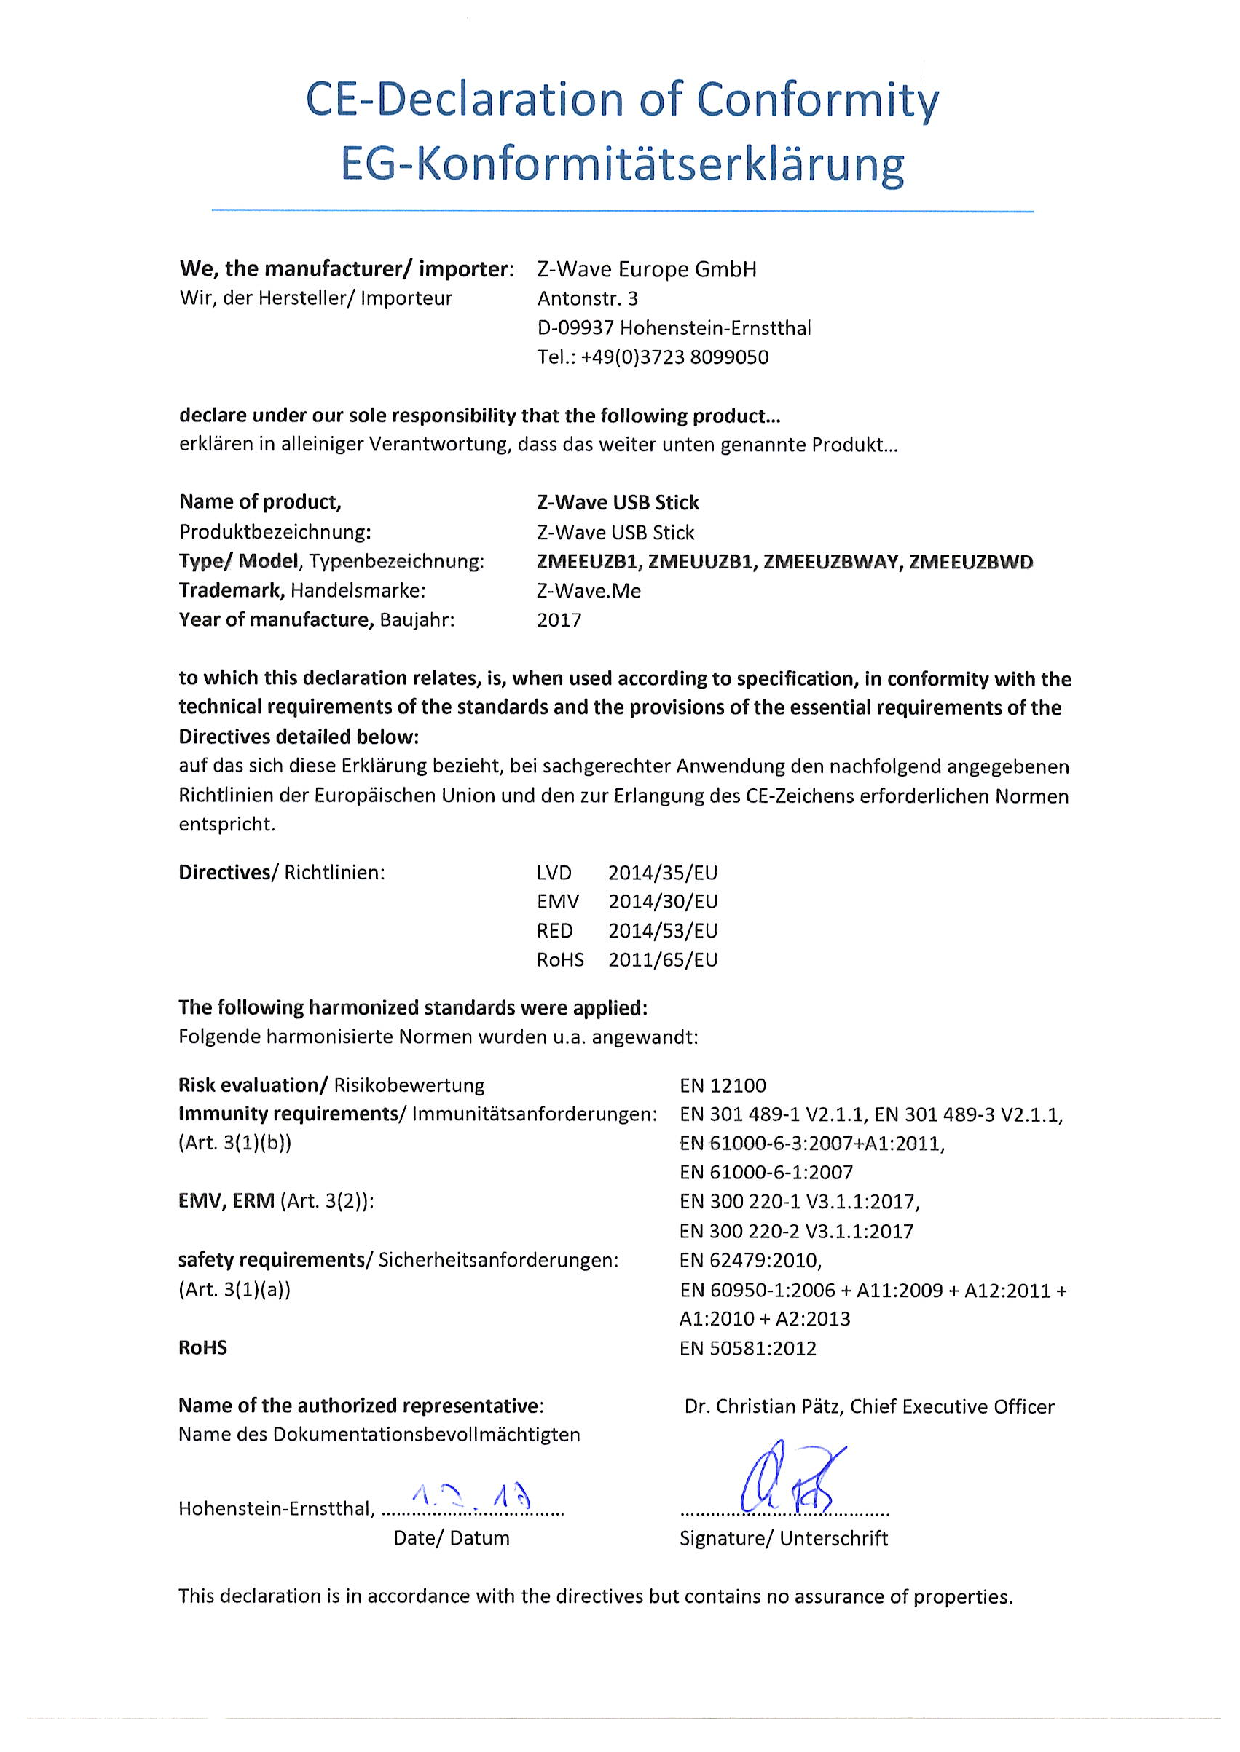
\includegraphics[width=0.9\textwidth]{pdfs/CE_UZB.pdf}
 
\chapter{User Interface Fundamentals - Slides}
\label{slides}


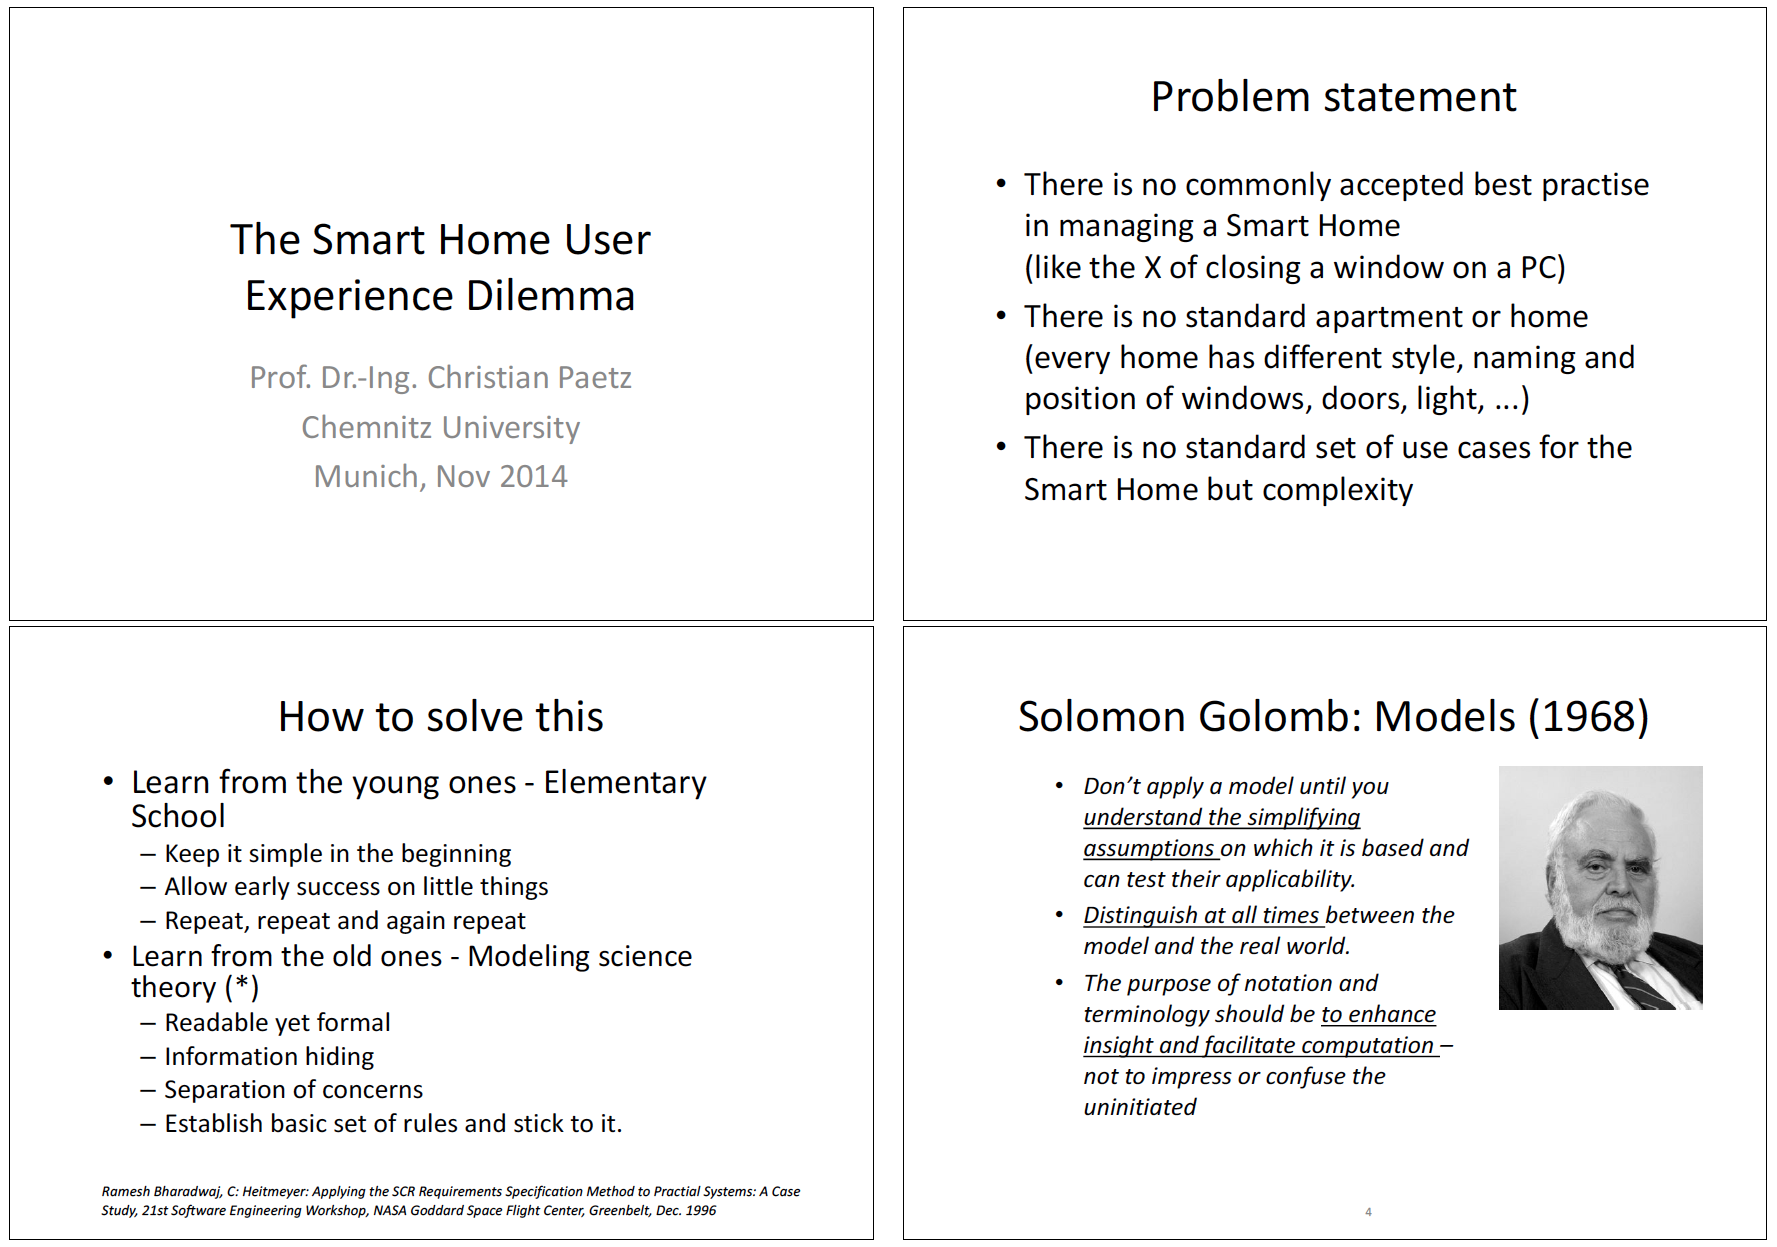
\includegraphics[width=0.9\textwidth]{pngs/funslides1.png}

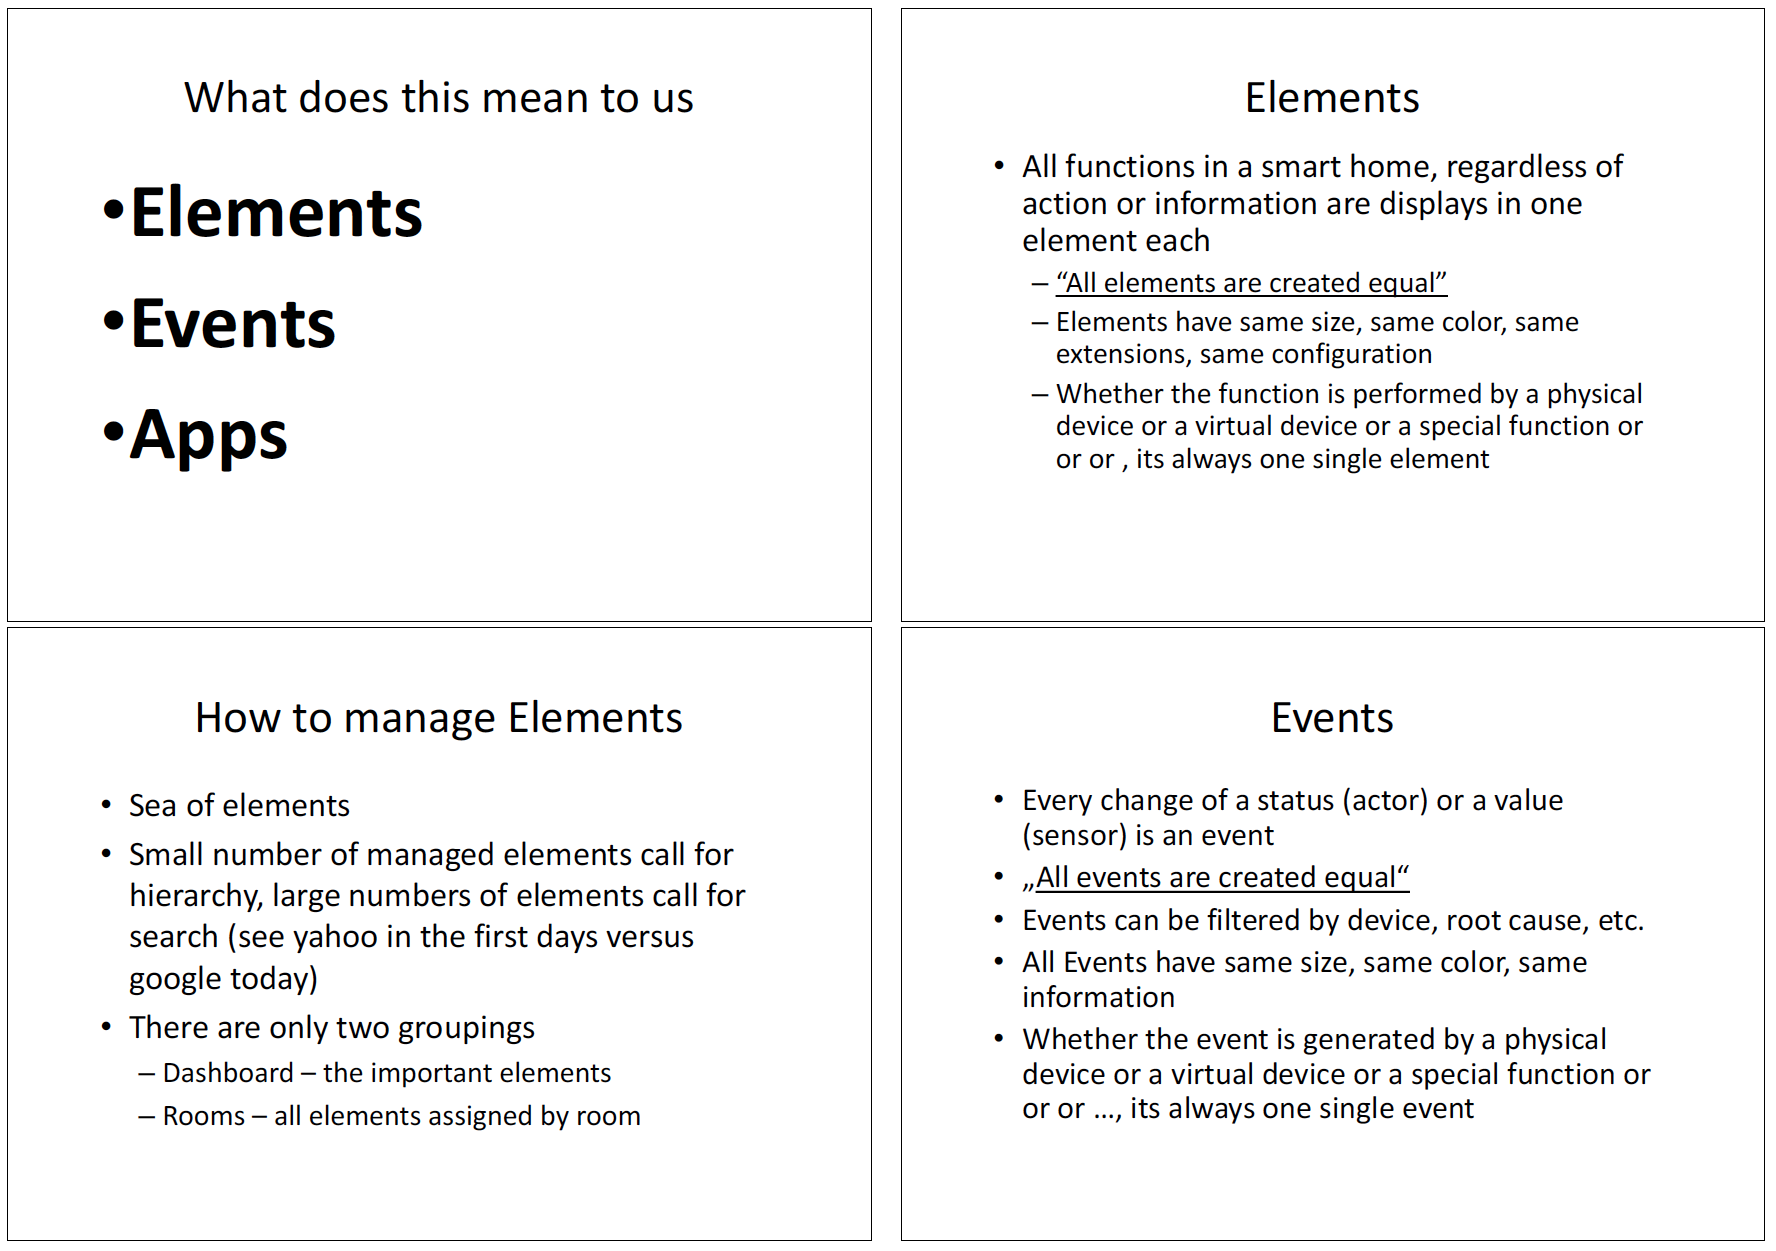
\includegraphics[width=0.9\textwidth]{pngs/funslides2.png}

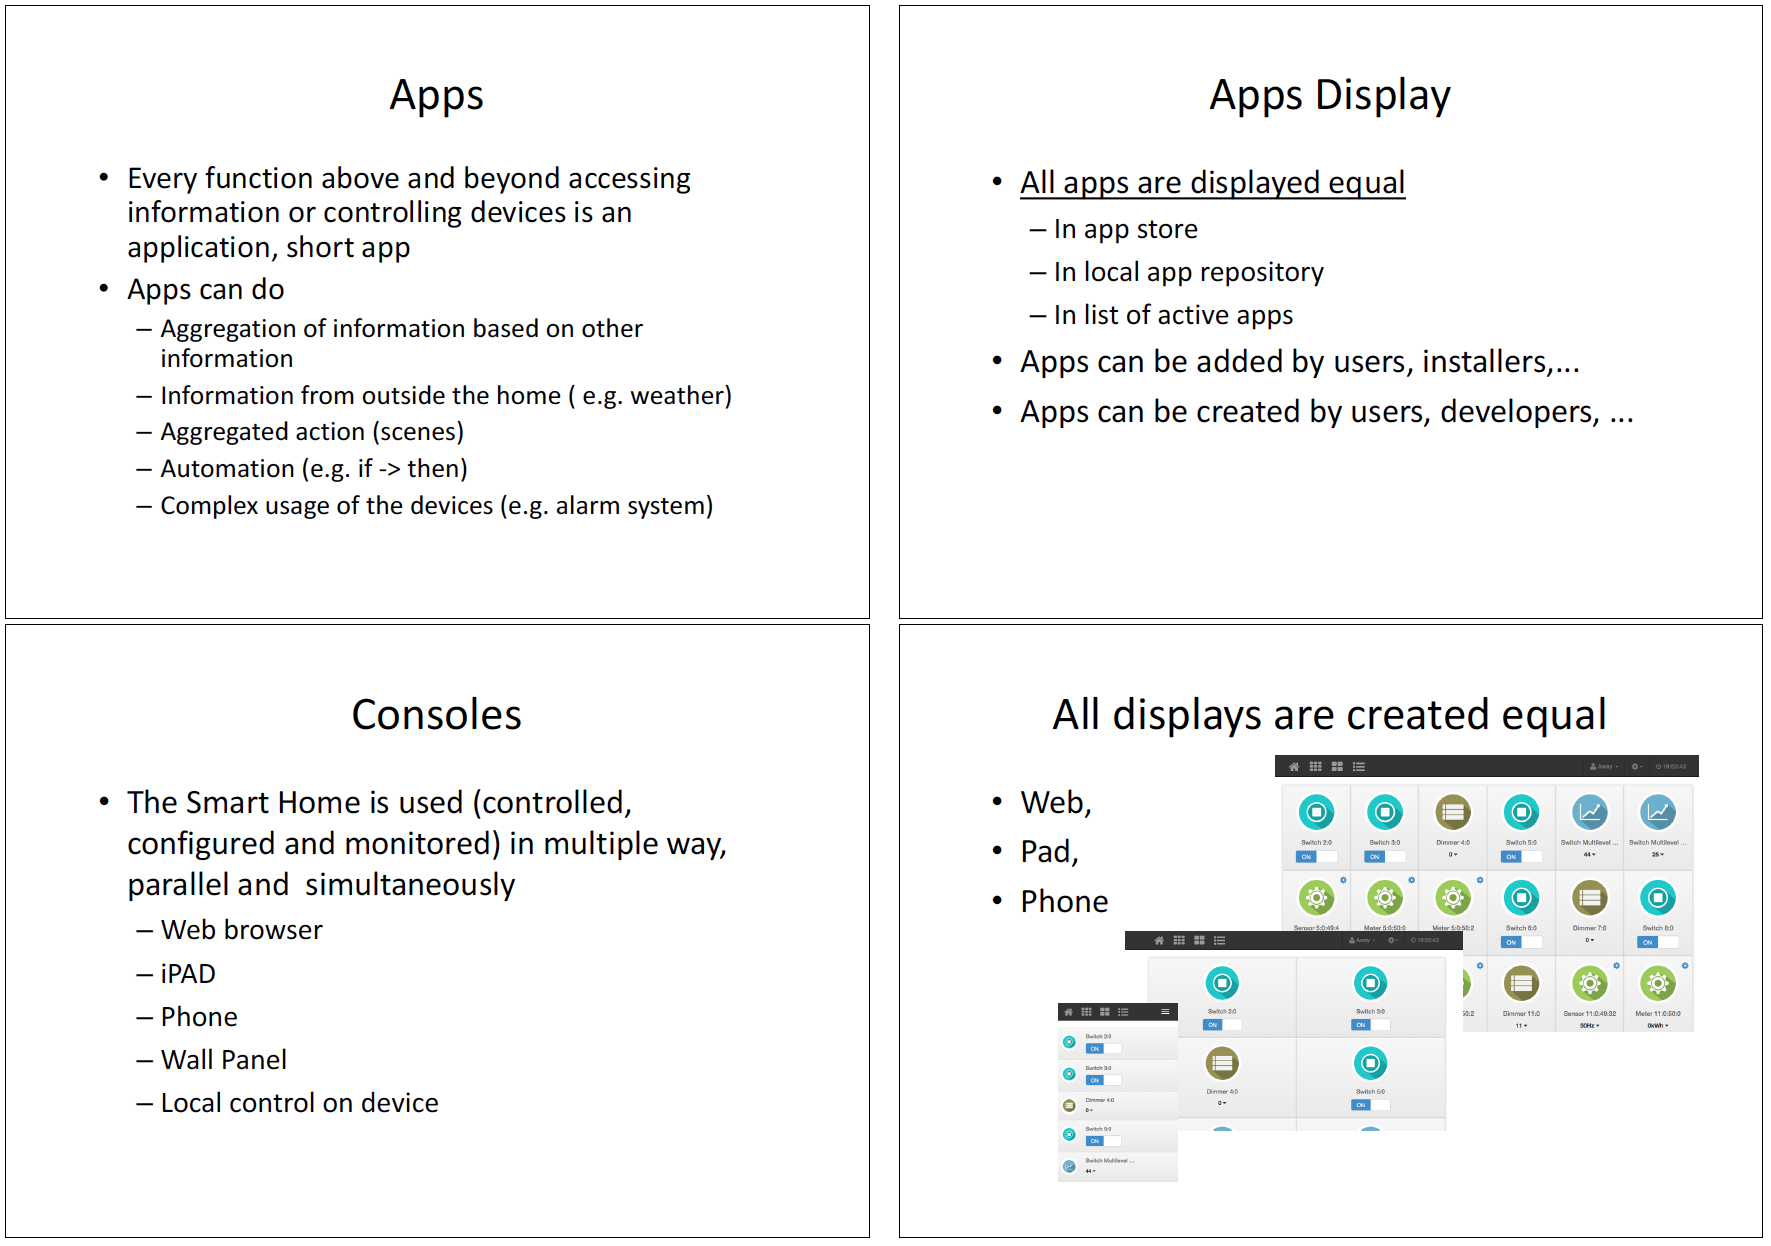
\includegraphics[width=0.9\textwidth]{pngs/funslides3.png}


\chapter{\zway Data Model Reference}
\label{annexdatamodel}

\section{Data}

This is the description of the data object (called Data Holder or DH).

General note: \zway objects and it's decendents are NOT simple JS objects, but native 
JS objects, that does not allow object modification.

\begin {itemize}
\item name: Name of data tree element
\item updated: Update time
\item invalidated: Invalidate time
\item valueOf(): Returns value of the object (can be omitted to get object value)
\item invalidate(): Invalidate data value (mark is as not valid anymore)
\item bind(function (type[, arg]) {...}, [arg, [watchChildren=false]]): Bind function 
to a change of data tree element of its descendants
\item unbind(function): Unbind function bind previously with bind()
\end {itemize}


\section{JS object zway}

\begin {itemize}
\item Description: zway is the Z-Wave part of the object tree
\item Syntax:  zway.X with  X as child object
\item Child objects
\begin {itemize}
\item controller: controller object, see below for details
\item devices: devices list, see below for details
\item version: Z-Way.JS version
\item isRunning(): Check if \zway is running
\item isIdle(): Check if \zway is idle (no pending packets to send)
\item discover(): Start \zway discovery process
\item stop() : Stop \zway
\item InspectQueue() : Returns list of pending jobs in the queue.
\begin {itemize}
\item item: [timeout, flags, nodeId, description, progress, payload]
\item flags: [send count, wait wakeup, wait security, done, wait ACK, got ACK, wait response, got response, wait callback, got callback]
\end {itemize}
\item ProcessPendingCallbacks(): Process pending callbacks (result of setTimeout/setInterval or functions called via HTTP JSON API)
\item bind(function, bitmask): Bind function to be called on change of devices list/instances list/command classes list
\item unbind(function) : Unbind function previously bind with bind()
\item all function classes in \ref{FunctionClasses} are also methods of this data object
\end {itemize}
\end {itemize}

\section{controller}

You can access the data elements of "controller" in the \zweui in menu 
\directory{Network > Controller Info} using the buttons \keystroke{Show controller data} 
and \keystroke{Show controller's device data.}

\begin {itemize}
\item Description: Controller object
\item Syntax: controller.X with  X as child object
\item Child objects
\begin {itemize}
\item data: Data tree of the controller
\begin {itemize}
\item  homeId: Home ID of the controller
\item  nodeId: Node ID of the controller
\item  SISPresent: is SIS available (if TRUE, SUCNodeId is a SIS, otherwise it is SUC)
\item  SUCNodeId: Node ID of SUC or SIS or 0 if no SUC/SIS present
\item  isInOtherNetworks: is controller the original Primary or it is in other's network
\item  isPrimary: can controller include devices (Primary or Inclusion controller)
\item  isRealPrimary: is controller Primary Controller or SIS in the network
\item  isSUC: is SUC present
\item  libType: Z-Wave library type
\item  frequency: current frequency of the transceiver

\item  controllerState: current network management state of the controller
\item  lastExcludedDevice: Node ID of last excluded device
\item  lastIncludedDevice: Node ID of last included device
\item  secureInclusion: shall inclusion be done using Security

\item  caps: \zway license information
\item  softwareRevisionVersion: version of \zway build
\item  softwareRevisonDate: date of \zway build
\item  softwareRevisionId: git commit of \zway build

\item  manufacturerId / manufacturerProductId / manufacturerProductTypeId: IDs to identify the transceiver hardware
\item  vendor: name of hardware vendor
\item  APIVersion: Version of the Serial API of the transceiver firmware
\item  SDK: Z-Wave SDK version of the transceiver firmware
\item  ZWVersion: ZWave Version (firmware)
\item  ZWaveChip: Serie of the transceiver Z-Wave chip
\item  ZWlibMajor / ZWlibMinor: library version 
\item  capabilities: array of Function Class IDs supported by the transceiver firmware
\item  functionClasses: ordered array of IDs of Function Classes
\item  functionClassesNames: ordered array of Names of Function Classes
\item  uuid: \zway transceiver firmware unique ID

\item  memoryGetAddress: address of last data stored in memoryGetData read by one of memory read function
\item  memoryGetData: last data read by one of memory read function
\item  countJobs: shall job be counted (nonManagementJobs and devices[x].data.queueLength)
\item  nonManagementJobs: number of non-management jobs in the queue
\item  deviceRelaxDelay: time in 10ms to wait before sending next command to same device (configurable in Defaults.xml)
\item  incomingPacket: last incoming packet from Z-Wave network

\item  curSerialAPIAckTimeout10ms: timing parameter of Serial API
\item  curSerialAPIBytetimeout10ms: timing parameter of Serial API
\item  oldSerialAPIAckTimeout10ms: previous timing parameter of Serial API
\item  oldSerialAPIBytetimeout10ms: previous timing parameter of Serial API
\end {itemize}

\end {itemize}
\end {itemize}

Function classes as shown in section \ref{FunctionClasses} are called als object functions of the 
data object zway.controller.


\section{Devices}

The devices object contains the array of the device objects. Each device in the network - including the 
controller itself -  has a device object in \zway.

\begin {itemize}
\item Description: list of devices
\item Syntax:  X with  X as child object
\item Child objects
\begin {itemize}
\item [m]: Device object
\item length: Length of the list
\item SaveData(): Save \zway Z-Wave data for hot start on next run (in config/zddx/HOMEID-DevicesData.xml)
\end {itemize}
\end {itemize}
 

\section{Device}

The data object can be accesses in the \zweui in advanced mode of 'Configuration'

\begin {itemize}
\item Description: the device object
\item Syntax:  device[n].X with  X as child object
\item Child objects
\begin {itemize}
\item id: (node) Id of the device
\item Data: Data tree of the device
\begin {itemize}
\item SDK: SDK used in the device firmware
\item ZDDXMLFile: file of the Devcie Description Record
\item ZWLib: Z-Wave library used in the device firmware
\item ZWProtocolMajor / ZWProtocolMinor: Z-Wave protocol version
\item applicationMajor / ApplicationMinor: Application Version of devices firmware
\item manufacturerId / manufacturerProductId / manufacturerProductTypeId: ids used to identify the device
\item basicType: Z-Wave Basic Type
\item genericType: Z-Wave Generic Type
\item specificType: Z-Wave Specific Type
\item deviceTypeString: verbal Z-Wave Device Class
\item vendorString: verbal vendor name

\item nodeInfoFrame: Node Information Frame (NIF) array
\item isListening: is always listening
\item isAwake: is currently awake
\item keepAwake: shall the device be kept awake even if there is nothing to send to it
\item isRouting: is abale to send routed unsolicited packets
\item sensor1000: device is a FLiRS with 1000 ms wakeup
\item sensor250: device is a FLiRS with 250 ms wakeup
\item isVirtual: is virtual device from a bridge controller
\item option: are optional Command Classes present in addition to mandatory for this Device Class
\item infoProtocolSpecific: internal information about the device
\item interviewDone: set to true when device finishes the interview (might not match with interviewDone on individual CCs if they appear after interview done)

\item neightbours: list of neighbour nodes

\item givenName: name for Expert UI
\item isFailed: is failed
\item failureCount: number of tries since last device failed
\item lastRecevied: timestamp of last packet received
\item lastSend: timestamp of last sent operation
\item lastPacketInfo: structure with deliveryTime, delivered and packetLength information about last packet sent
\item queueLength: length of device specific send queue (if countJobs is enabled)
\item lastNonceGet: internal
\end {itemize}

\item instances: iInstances list of the device
\item RequestNodeInformation(): Request NIF
\item RequestNodeNeighbourUpdate(): Request routes update
\item InterviewForce(): Purge all command classes and start interview based on device's NIF
\item RemoveFailedNode(): Remove this node as failed. Device should be marked as failed to remove it with this function.
\item SendNoOperation(successCallback = NULL, failureCallback = NULL): Ping the device with empty packet (even if device is not reachable successCallback is called - use isFailed to check device availability)
\item LoadXMLFile(file): Load new Z-Wave Device Description XML file. See http://pepper1.net/zwavedb/
\item GuestXML(): Return the list of all known Z-Wave Device Description XML files with match score. [score, file name, brand name, product name, photo]
\item WakeupQueue(): Pretend the device is awake and try to send packets
\item AssignReturnRoute(target): Send device new routes to target node
\item DeleteReturnRoute(): Clear routes in device
\item AssignSUCReturnRoute(): Inform device about SUC and route to reach it
\end {itemize}
\end {itemize}

\section{Instances}

Each device may have multiple instances (similar functions like switches, same type 
sensors, ...) If only one instance is present the id of this instance is 0. Command 
classes are located in instances only.

\begin {itemize}
\item Description: list of instances
\item Syntax:  device[n].instance[m].X with  X as child object
\item Child objects
\begin {itemize}
\item [m]: instance object
\item length: Length of the list
\item commandClasses: list of command classes of this instance. In case there is only one instance, this is equivalent to the list of command classes of the device. For details see below.
\item Data: data object of instance 
\begin {itemize}
\item dynamic: flag if instance is dynamic
\item genericType: generic Z-Wave device class of instance
\item specificType: specific Z-Wave device class of instance
\end {itemize}
\end {itemize}
\end {itemize}

\section{CommandClass}

This is the Command Class object. It contains public methods and public data elements that are described
in chapter \ref{ccs}

\begin {itemize}
\item Description: Command Class Implementation
\item Syntax:  device[n].instance[m].commandclass[id].X with  X as child object
\item Child objects
\begin {itemize}
\item id: Id of the Command Class of the instance of the device
\item data: Data tree of the Command Class
\begin {itemize}
\item interviewCounter: number of attempts left until interview is terminate even if not successful
\item interviewDone: flag if interview of the command class is finished
\item security: flag if Command Class is operated under Security Command Class
\item version: version of the Command Class implemented in the device
\item supported: flag if Command Class is supported or only controlled
\item {commandclass data}: Command Class specific data - see chapter \ref{ccs} for details.
\end {itemize}
\item name: Command Class name
\item {Method}: Command Class method - see chapter \ref{ccs} for details.
\end {itemize}
\end {itemize}


 
